\documentclass[{../../master}]{subfiles}
\graphicspath{{../..}}  % 個別コンパイル時の画像パスを解決する

\begin{document}

\section{\textsf{wheel\_link}の作成と追加}

最後に\textsf{wheel\_link}とそのジョイントを追加していきます.
\textsf{wheel\_link}を定義するために2つのファイルを準備します.
\textsf{wheel.xacro}と\textsf{transmission.xacro}の2つです.

\subsection{\textsf{wheel.xacro}の作成}

まずは\textsf{wheel.xacro}を記述していきます.
\textsf{urdf/}ディレクトリ以下に\textsf{wheel/}ディレクトリを作成し,\textsf{wheel.xacro}という名前のファイルを作成します.
そして,コード\ref{code:wheel_xacro}のように記述します.

\begin{lstlisting}[language=XML, label=code:wheel_xacro, caption=\textsf{wheel.xacro}]
<?xml version="1.0"?>
<robot xmlns:xacro="http://ros.org/wiki/xacro">
  <xacro:macro name="wheel" params="prefix parent *joint_origin *joint_axis">
    <joint name="${prefix}_wheel_joint" type="continuous">
      <xacro:insert_block name="joint_origin"/>
      <parent link="${parent}"/>
      <child link="${prefix}_wheel_link"/>
      <xacro:insert_block name="joint_axis"/>
    </joint>
    
    <link name="${prefix}_wheel_link">
      <visual>
        <origin rpy="0.0 0.0 0.0"/>
        <geometry>
          <mesh filename="package://adamr2_description/meshes/wheel_link.STL"/>
        </geometry>
        <material name="black">
          <color rgba="0.0 0.0 0.0 1.0"/>
        </material>
      </visual>
    </link>
  </xacro:macro>
</robot>
\end{lstlisting}

\textsf{wheel.xacro}の内容は他のリンクとほとんど変わり映えしません.
ジョイントとリンクを定義しているだけです.
ホイールを繋ぐジョイントはタイプを\textsf{continuous}にします.

\subsection{\textsf{transmission.xacro}の作成}

ホイールジョイントに対する\textsf{ros\_control}の設定を行うマクロは\textsf{transmision.xacro}で定義します.
\textsf{wheel.xacro}と同じディレクトリに\textsf{transmission.xacro}という名前のファイルを作成し,コード\ref{code:transmission_xacro}のような内容を記述します.

\begin{lstlisting}[language=XML, label=code:transmission_xacro, caption=\textsf{transmission.xacro}]
<?xml version="1.0"?>
<robot xmlns:xacro="http://ros.org/wiki/xacro">
  <xacro:macro name="wheel_trans" params="prefix">
    <transmission name="${prefix}_wheel_trans">
      <type>transmission_interface/SimpleTransmission</type>
      <joint name="${prefix}_wheel_joint">
        <hardwareInterface>hardware_interface/VelocityJointInterface</hardwareInterface>
      </joint>

      <actuator name="${prefix}_wheel_motor">
        <mechanicalReduction>1</mechanicalReduction>
      </actuator>
    </transmission>
  </xacro:macro>
</robot>
\end{lstlisting}

このマクロではホイールのジョイントに対して\textsf{transmission}要素を追加しています.
\textsf{transmission}要素には\textsf{type},\textsf{joint},\textsf{actuator}の3つの要素を持っています.
このURDFは\textsf{ros\_control}のコントローラの1つである\textsf{diff\_drive\_controller}から利用されることを想定しているので,
\textsf{type}は\textsf{transmission\_interface/SimpleTransmission}を,
\textsf{joint}の\textsf{hardwareInterface}要素には\textsf{hardware\_interface/VelocityJointInterface}を設定しています.
\textsf{actuator}要素の\textsf{mechanicalReduction}には,ロボットのアクチュエータの減速比を設定します.
ADAMR2ではギヤードBLDCモータを使用していますが,ギア比の計算はYP-Spurが行ってくれるため,ここで設定する必要はありません.
ギヤ比は1に設定しておきましょう.

\subsection{ルートファイルからインクルードする}

ホイールをロボットに組み込みます.\textsf{robot.xacro}を更に編集し,コード\ref{code:robot_xacro_add_wheel_link}のようにします.
\textsf{xacro:include}タグを使って\textsf{wheel.xacro}と\textsf{transmission.xacro}を読み込むことを忘れないようにしてください.

\begin{lstlisting}[language=XML, label=code:robot_xacro_add_wheel_link, caption=Add \textsf{wheel\_link} to Robot Model]
<?xml version="1.0"?>
<robot name="adamr2" xmlns:xacro="http://ros.org/wiki/xacro">
  <xacro:include filename="$(find adamr2_description)/urdf/base/base.xacro"/>
  <xacro:include filename="$(find adamr2_description)/urdf/caster/caster.xacro"/>
  <xacro:include filename="$(find adamr2_description)/urdf/lidar/lidar.xacro"/>
  <xacro:include filename="$(find adamr2_description)/urdf/wheel/wheel.xacro"/>
  <xacro:include filename="$(find adamr2_description)/urdf/wheel/transmission.xacro"/>

  <!-- base_footprint -->
  <link name="base_footprint"/>

  <!-- base_link -->
  <xacro:base parent="base_footprint">
    <origin xyz="0.0 0.0 0.262"/>
  </xacro:base>

  <!-- front caster -->
  <xacro:caster prefix="front" parent="base_link">
    <origin xyz="0.275 0.0 -0.1498" rpy="0 0 ${radians(180)}"/>
  </xacro:caster>

  <!-- back caster-->
  <xacro:caster prefix="back" parent="base_link">
    <origin xyz="-0.275 0.0 -0.1498"/>
  </xacro:caster>

  <!-- lidar -->
  <xacro:lidar parent="base_link" visual_yaw_orientation="${radians(180)}">
    <origin xyz="0.275 0 0.177" rpy="0 0 ${radians(270)}"/>
  </xacro:lidar>

  <!-- left wheel -->
  <xacro:wheel prefix="left" parent="base_link">
    <origin xyz="0.0 0.1915 -0.1845"/>
    <axis xyz="0 1 0"/>
  </xacro:wheel>
  <xacro:wheel_trans prefix="left"/>

  <!-- right wheel -->
  <xacro:wheel prefix="right" parent="base_link">
    <origin xyz="0.0 -0.1915 -0.1845"/>
    <axis xyz="0 1 0"/>
  </xacro:wheel>
  <xacro:wheel_trans prefix="right"/>
</robot>
\end{lstlisting}

\textsf{xacro:wheel}を呼び出してホイールを定義しています.
ここで重要なのが,ホイールの回転軸は「ロボットが直進する方向を正とする」ようにしなければならないということです.
コード\ref{code:robot_xacro_add_wheel_link}を見るとわかるように,左右どちらの車輪も,Y軸正方向を回転軸に設定しています.
これは\textsf{diff\_drive\_controller}を使用する都合で発生するものです.
\footnote{後述しますが,YP-Spurにおける車輪の軸はこのようになっていないため,結局ドライバノード側で回転速度を反転しなければなりません.にも関わらずこのようにしているのは,できるだけシミュレーション環境と互換性を持たせるためです.}

\subsection{\textsf{rviz}による可視化}

駆動パーツであるホイールを追加したので,\textsf{rviz}で可視化して,ついでにジョイントを動かしてみましょう.
\textsf{joint\_state\_publisher\_gui}パッケージを使用すれば,スライダーを使ってジョイントを動かすことができます.
\textsf{joint\_state\_publisher\_gui}パッケージはデフォルトで入っていない場合があるので,追加でインストールします.

\begin{lstlisting}[language=sh, caption=Install \textsf{joint\_state\_publisher\_gui}]
sudo apt update
sudo apt install ros-melodic-joint-state-publisher-gui
\end{lstlisting}

\textsf{display.launch}に\textsf{joint\_state\_publisher}と\textsf{joint\_state\_publisher\_gui}を起動する文を追加します.

\begin{lstlisting}[language=XML, label=code:display_launch_add_joint_state_publisher_gui, caption=\textsf{display.launch}]
<launch>
  <arg name="model" default="$(find adamr2_description)/urdf/robot.xacro"/>
  <arg name="rvizconfig" default="$(find adamr2_description)/rviz/display.rviz" />

  <param name="robot_description" command="$(find xacro)/xacro $(arg model)" />

  <node name="robot_state_publisher" pkg="robot_state_publisher" type="robot_state_publisher"/>
  <node name="joint_state_publisher_gui" pkg="joint_state_publisher_gui" type="joint_state_publisher_gui"/>
  <node name="rviz" pkg="rviz" type="rviz" args="-d $(arg rvizconfig)" required="true"/>
</launch>
\end{lstlisting}

これを実行すると,図\ref{fig:rviz_joint_state_publisher_gui}のように,\textsf{rviz}にロボットモデルが表示され,また\textsf{joint\_state\_publisher\_gui}のウィンドウが現れます.
\textsf{joint\_state\_publisher\_gui}のウィンドウのスライダーをマウスで動かすことによって,\textsf{rviz}上のロボットのホイールも動きます.
ジョイントの角度を正の数値にすると,ロボットが前進する方向へホイールが動くことを確認してください.

\begin{figure}[ht]
  \centering
  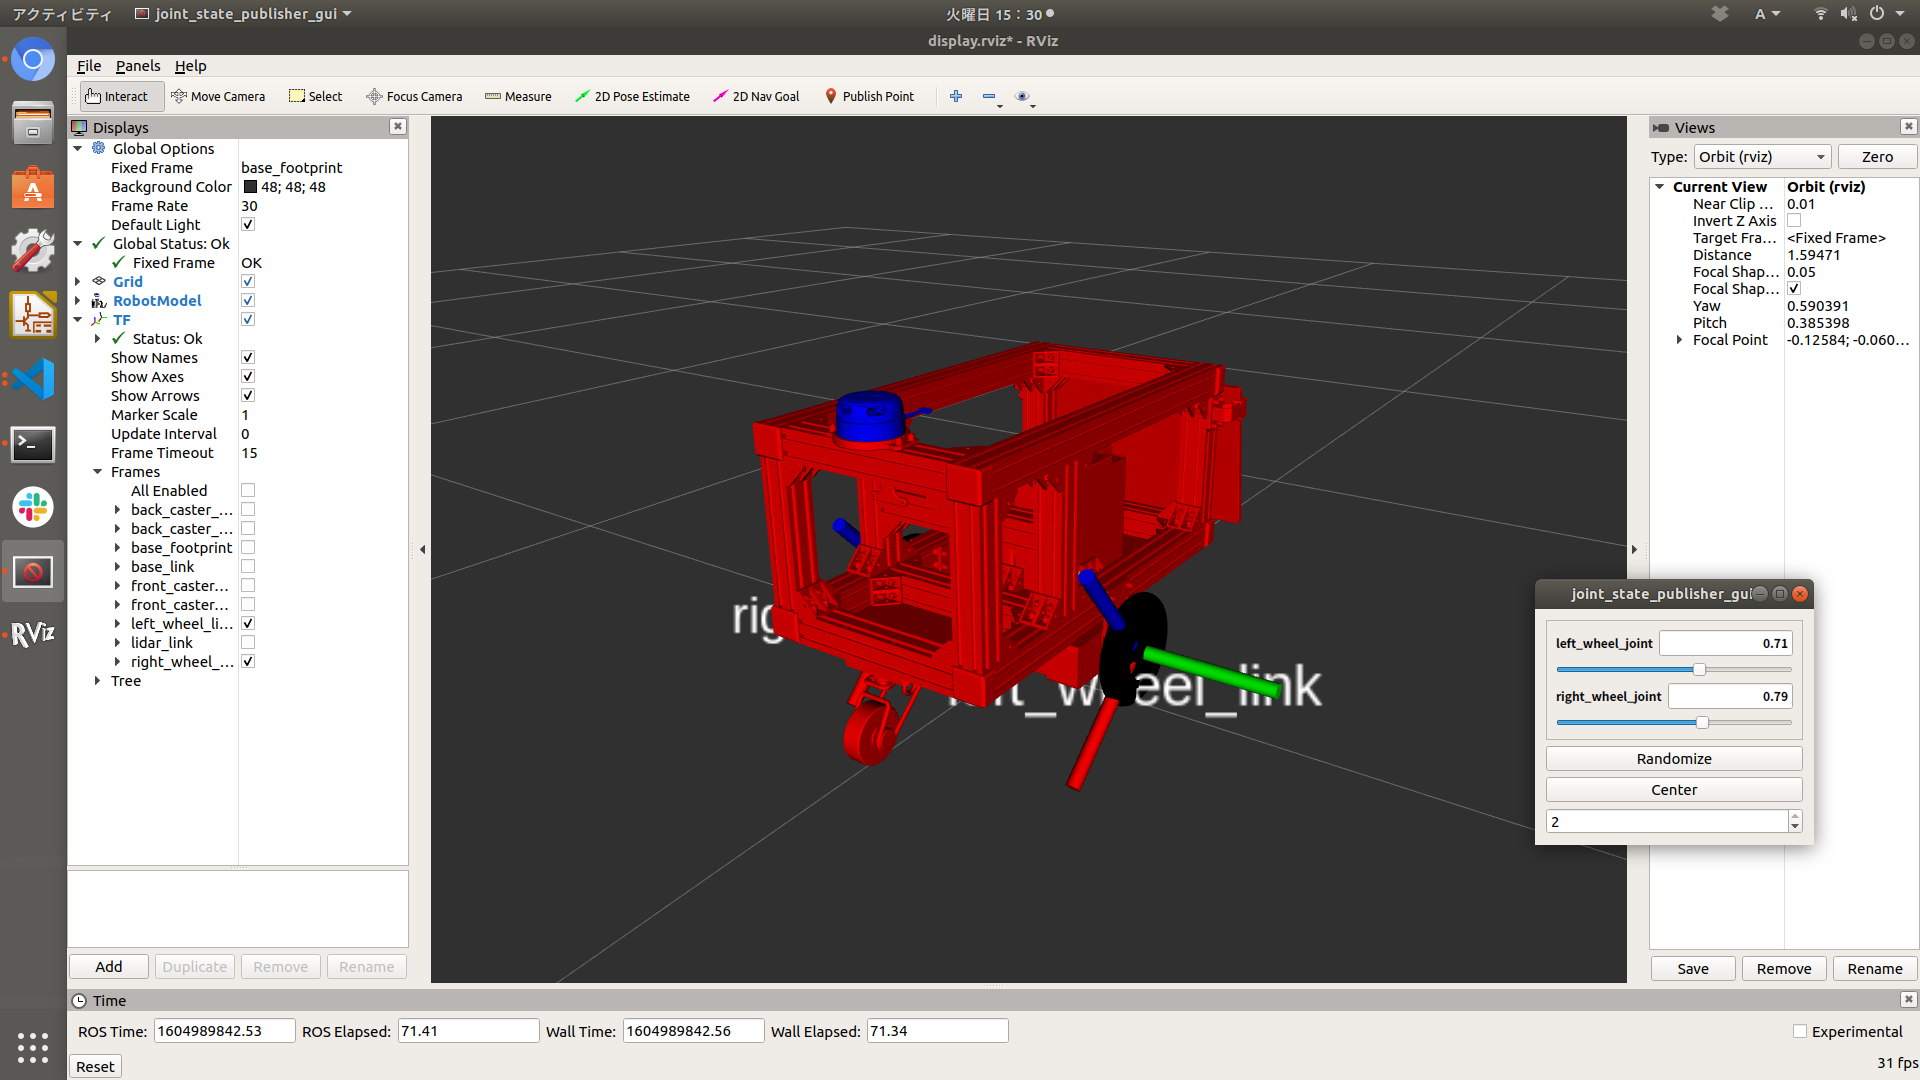
\includegraphics[width=120truemm]{images/rviz_joint_state_publisher_gui.png}
  \label{fig:rviz_joint_state_publisher_gui}
  \caption{\textsf{joint\_state\_publisher\_gui}}
\end{figure}

\end{document}